\chapter{\uppercase{metode penelitian}} \label{metode_penelitian}
Metode penelitian membahas segala sesuatu yang dilakukan untuk mencapai tujuan. Bab ini minimal berisi alat-alat yang digunakan, baik \textit{hardware} maupun \textit{software}, bahan yang dipakai, dan langkah-langkah penelitian.

\section{Tempat dan Waktu}
Tuliskan tempat dan waktu pelaksanaan penelitian saudara.

\section{Alat Penelitian}
Sebutkan alat-alat yang dipakai beserta spesifikasinya. Jika diperlukan disertai dengan kegunaannya. Alat yang dipakai dalam penelitian ini adalah:
\begin{enumerate}
	\item Komputer 2 buah.\\
	Komputer ini satu digunakan sebagai client dan satu sebagai server. dan seterusnya dan seterusnya.
	\item Laptop
	\item MATLAB (semua alat di muka adalah contoh)
\end{enumerate}

\section{Bahan Penelitian}
Sebutkan bahan penelitian yang dipakai. Anda harus dapat membedakan antara alat dan bahan. Alat adalah perangkat untuk mengolah bahan, sedangkan bahan adalah yang diolah. Data penelitian dapat dimasukkan sebagai bahan, atau dapat dibuat subbab tersendiri. Sebutkan ada berapa data, dan diambil dari mana dan/atau bagaimana cara memperolehnya.

\section{Rencana Penelitian}
Sebutkan langkah-langkah penelitian yang akan ditempuh untuk meraih tujuan penelitian yang ingin dicapai (lihat Tujuan di Bab 1. Ungkapkan dalam bentuk gambar flowchart. Jelaskan maksud flowchart anda. Gambar \ref{langkahpenelitian} adalah contoh langkah-langkah penelitian.
	\begin{figure}
		\centering
		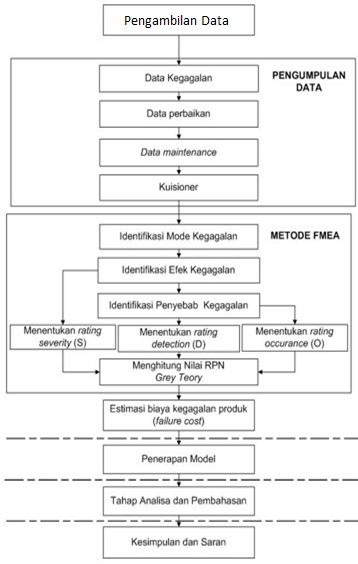
\includegraphics{langkahpenelitian}
		\caption{Langkah Penelitian}
		\label{langkahpenelitian}
	\end{figure}
	
	Tidak perlu menyertakan studi literatur di dalam langkah penelitian. Studi literatur sudah jelas dilakukan pada setiap penelitian apapun. Jelaskan masing-masing tahapan pada Gambar \ref{langkahpenelitian} yang dilakukan. Jelaskan tahapan-tahapan ini dalam subsection yang berurutan.
	
	Selain langkah penelitian, gambar sistem yang dirancang perlu digambarkan. Gambar sistem harus disertakan ketika penelitian mengandung unsur perancangan sistem. Gambar \ref{perancagansistem} adalah contoh gambar sistem.
	\begin{figure}
		\centering
		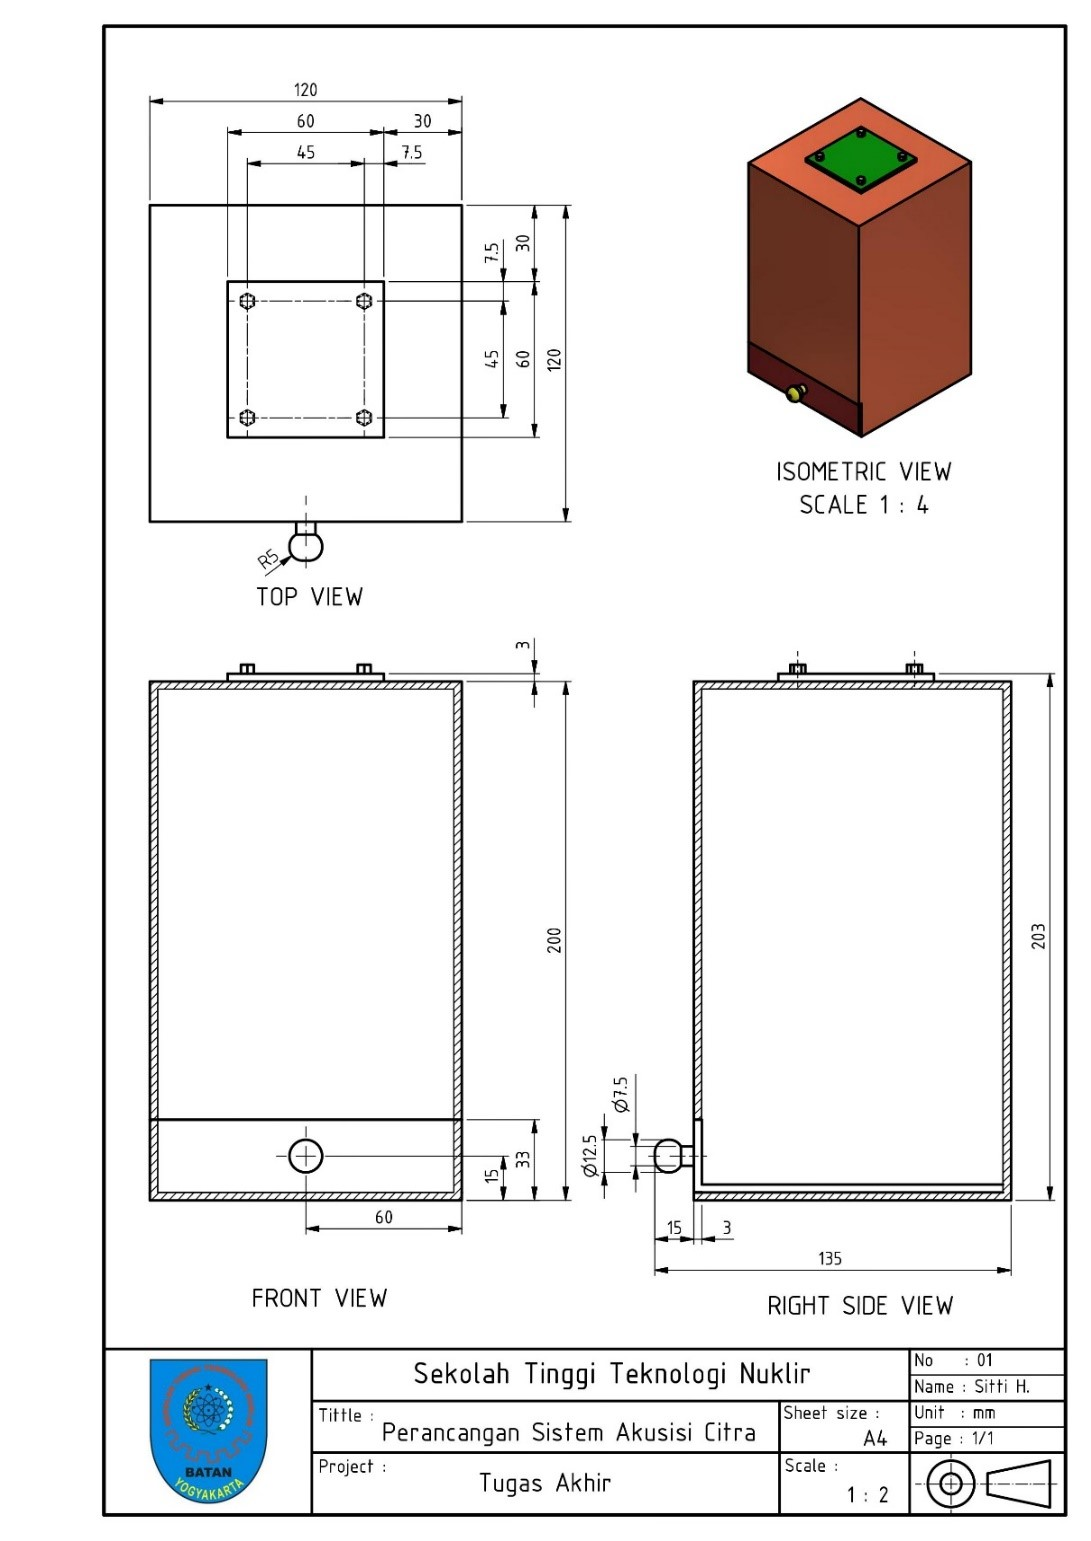
\includegraphics{perancangan_sistem}
		\caption{Perancangan Sistem}
		\label{perancagansistem}
	\end{figure}
	
	Gunakan simbol diagram yang tepat. Jelaskan makna Gambar \ref{perancagansistem} secara keseluruhan, serta jelaskan makna masing-masing bagiannya
	
	Ungkapkan hal-hal lain dalam penelitian jika dirasakan perlu. Hal-hal yang perlu diungkapkan mungkin saja berupa kesulitan-kesulitan, keterbatasan alat, kesulitan pengambilan data, dan lain-lain. Sebutkan bagaimana cara mengatasi atau skenario ketika gagal karena kesulitan/keterbatasan tersebut. Hal lain ini dapat juga berupa modal penelitian sebelumnya yang berhasil.
	
	Pada Bab ini selain dijelaskan cara perancangan dan pembuatan juga harus dijelaskan cara analisis (metode pengujian) yang akan dilakukan.
	
	\section{Metode Analisis}
	Tuliskan langkah-langkah dalam melakukan analisis. Langkah-langkah ini harus dilandasi di section 2.2. \ref{rumus}